\documentclass[a4paper,runningheads]{llncs}

\usepackage[T1]{fontenc}
\usepackage{graphicx,color}
\usepackage{amsmath,amssymb,amsfonts}
\usepackage{booktabs}
\usepackage{array}
\usepackage{multirow}
\usepackage{makecell}
\usepackage{algorithm}
\usepackage{algpseudocode}
\usepackage{enumitem}
\usepackage{xcolor}
\usepackage{tikz}
\usepackage{pgfplots}
\usepackage{url}
\usepackage[hidelinks]{hyperref}

\usetikzlibrary{arrows.meta,positioning,calc,fit,shapes.geometric,backgrounds}
\pgfplotsset{compat=1.17}

\newcommand{\Fp}{\mathbb{F}_p}
\newcommand{\Fq}{\mathbb{F}_q}
\newcommand{\ZZ}{\mathbb{Z}}
\newcommand{\RR}{\mathbb{R}}
\newcommand{\supp}{\operatorname{supp}}
\newcommand{\Eval}{\operatorname{Eval}}
\newcommand{\ord}{\operatorname{ord}}
\newcommand{\Span}{\operatorname{span}}
\newcommand{\HElib}{\textsf{HElib}}
\newcommand{\BGV}{\textsf{BGV}}
\newcommand{\BFV}{\textsf{BFV}}
\newcommand{\CKKS}{\textsf{CKKS}}
\newcommand{\GBFV}{\textsf{GBFV}}
\newcommand{\Sat}{\textsf{SAT}}
\newcommand{\Aopt}{256}
\newcommand{\Abase}{35}
\newcommand{\termsbase}{612}
\newcommand{\termsopt}{307}
\newcommand{\degclean}{1223}
\newcommand{\supportsize}{1225}

\begin{document}

\title{Character-Filtered Exact Cleaners and Galois-Structured Design for Large-Prime BGV Bootstrapping}
\titlerunning{Character-Filtered Exact Cleaners for BGV Bootstrapping}

\author{Anonymous Authors}
\authorrunning{Anonymous Authors}
\institute{Anonymous Institution}

\maketitle

\begin{abstract}
Large-prime \BGV bootstrapping recently became practical by combining bounded-support null-polynomial reductions over $\mathbb{Z}_{p^e}$. We study the next structural layer inside that improved pipeline. For a fixed bounded support $S_A=\{hA+\ell\bmod p : h,\ell\in[-B,B]\}$, the exact cleaner $P_A(hA+\ell)=\ell$ has a unique degree-$<|S_A|$ representative in the support quotient. Hence, after bounded-support degree reduction, the remaining stable objective is not lower degree for the same support, but lower encrypted polynomial-evaluation cost.

Our main result is an implemented order-four cleaner for the target large-prime parameter set $p=65537$, $B=17$. We find and certify the radix $A=256$ with $A^2=-1\bmod p$. This makes the support stable under a quarter-turn and forces the canonical cleaner to satisfy $P_A(AX)+AP_A(X)=AX$. Equivalently, the monomial basis of the support quotient decomposes into finite-field character spaces, and all exponents except $X$ and $k\equiv3\pmod4$ vanish. The resulting exact cleaner keeps the same minimum degree $1223$ as the generic baseline radix $A=35$, but its nonzero monomial count drops from $612$ to $307$. We implement this cleaner and its specialized evaluator in an isolated \HElib artifact. In real ciphertext thin bootstrapping, digit extraction drops from $160.783$~s to $80.770$~s and full thin bootstrapping from $213.103$~s to $131.181$~s, speedups of $49.76\%$ and $38.44\%$ over the direct large-prime baseline.

Beyond the implemented order-four case, we give two conservative extensions. First, we formulate an order-adaptive cleaner planner. For $p=65537$, order four is the stable global choice at $B=17$, whereas order eight becomes support-safe only once the local support radius drops to $B\le7$, and order sixteen only for tiny local supports. These claims are supported by exact offline interpolation and evaluation-cost sweeps, not by a new ciphertext implementation. Second, we reinterpret the dominant EvalMap block in the target square-free cyclotomic index $m=50731=97\cdot523$ as a group-matrix problem. For the $D=96$ block, an exact plaintext Rader/FFT factorization reduces the operation count to $0.703\times$ the dense primitive-Vandermonde path. The current ciphertext transform integrations remain negative or engineering-only evidence, so we state this part as design guidance rather than as a second demonstrated speedup.

\keywords{Fully homomorphic encryption \and BGV bootstrapping \and Null polynomials \and Digit extraction \and Exact polynomial synthesis \and Galois structure \and Homomorphic linear transforms \and HElib}
\end{abstract}

% ================================================================
\section{Introduction}
\label{sec:intro}
% ================================================================

Large-prime \BGV bootstrapping is now practical because bounded-support null-polynomial methods drastically reduce the degree of the nonlinear cleaning step~\cite{ma_large_p}. The natural next question is what remains to optimize once that degree reduction has already been obtained.

This paper argues that the next stable optimization layer is \emph{structural}, not another attempt to beat the fixed-support degree minimum. For an auxiliary radix $A$, define the bounded support
\[
  S_A=\{hA+\ell\bmod p : h,\ell\in[-B,B]\},
  \qquad
  C_A(hA+\ell)=\ell.
\]
If the map $(h,\ell)\mapsto hA+\ell$ is injective, then the cleaner has a unique canonical representative $P_A$ of degree $<|S_A|$. Therefore, once the support is fixed, there is generally no remaining degree freedom to exploit. The remaining freedom is to choose a support geometry whose canonical representative is cheaper to evaluate homomorphically.

Our main observation is that the auxiliary radix controls this geometry. The implemented case is $A=256\in\mathbb{F}_{65537}^\times$, which satisfies $A^2=-1\bmod p$. Then multiplication by $A$ acts on support coordinates as the quarter-turn $(h,\ell)\mapsto(\ell,-h)$, and the cleaner obeys
\[
  P_A(AX)+AP_A(X)=AX.
\]
In the monomial basis, this identity is a character filter: only the monomial $X$ and exponents $k\equiv3\pmod4$ survive. As a result, the exact cleaner keeps the same minimum degree as the generic baseline but becomes much sparser. For $p=65537$, $B=17$, the term count drops from $612$ to $307$, and in a real \HElib artifact the resulting specialized evaluator reduces extraction from $160.783$~s to $80.770$~s and the full thin bootstrap from $213.103$~s to $131.181$~s.

This order-four result is the paper's only positive ciphertext algorithmic claim. We then use it as the first implemented point of a broader, conservatively stated framework. First, because $(\mathbb{Z}/p\mathbb{Z})^\times$ is cyclic, one can ask when higher subgroup order becomes support-safe. For the target prime $65537$, our exact offline sweep shows that order four is the stable global choice at $B=17$, while order eight becomes support-safe for smaller local supports such as $B\le7$, and order sixteen only for tiny local supports. Second, the same Galois structure appears on the linear-transform side. For the target square-free cyclotomic index $m=50731=97\cdot523$, the main transform block has size $D=96$, and an exact plaintext Rader/FFT factorization reduces arithmetic work to $0.703\times$ the dense primitive-Vandermonde path. However, the current ciphertext transform integrations remain negative or engineering-only evidence, so we present that part as design guidance rather than as a second speedup claim.

The paper's message is therefore deliberately asymmetric. It gives one fully implemented and benchmarked algorithmic result --- the order-four cleaner and its evaluator --- and uses exact offline search, exact plaintext verification, and negative ciphertext evidence to delimit a larger Galois-structured design space around it.

\paragraph{Claim boundary.}
The positive ciphertext claim is specific to a fixed \HElib large-prime \BGV thin-bootstrapping pipeline with the implemented order-four cleaner and evaluator. Higher-order cleaners and Galois-structured linear transforms are presented as exact theory, offline planner evidence, exact plaintext verification, and negative/guardrail ciphertext experiments. The paper does not claim a globally optimal bootstrapping pipeline or a demonstrated ciphertext speedup from the new linear-transform algebra.

\paragraph{Contributions.}
\begin{enumerate}[leftmargin=*,label=\textbf{\arabic*.}]
  \item \textbf{Character-filtered exact-cleaner formulation.}
  We formulate bounded-support large-prime cleaning in the support quotient and show that, after fixed-support degree reduction, the stable optimization target is sparsity and encrypted evaluation cost rather than a lower degree for the same support.

  \item \textbf{Implemented order-four cleaner and evaluator.}
  We prove the order-four cleaner identity $P_A(AX)+AP_A(X)=AX$ for $A^2=-1\bmod p$, derive the support restriction $P_A(X)=\frac12X+X^3Q(X^4)$, and implement this path in an isolated \HElib artifact. The repeat-three ciphertext benchmark gives a $49.76\%$ extraction speedup and a $38.44\%$ full thin-bootstrapping speedup over the direct large-prime baseline.

  \item \textbf{Order-adaptive cleaner theory.}
  We give a conservative higher-order generalization based on subgroup action, signed-circulant support models, and support-safety thresholds. For $p=65537$, the resulting planner shows that order four is the stable global choice at $B=17$, whereas order eight becomes support-safe only once the support radius is sufficiently smaller.

  \item \textbf{Galois-structured transform design route.}
  We reinterpret the main EvalMap blocks through the cyclotomic Galois group and a normal-basis / character-factorized matrix model. For the target $m=50731=97\cdot523$, we identify the $D=96$ block as the promising structured target, support that claim with exact plaintext Rader/FFT verification, and explain why $D=29$ is not the first optimization target.

  \item \textbf{Co-design boundary.}
  We use the existing negative and engineering-only linear-transform results to delimit the paper's scope and to frame transform support shaping and feasible cleaner order as a single co-design objective without overclaiming a second positive ciphertext route.
\end{enumerate}

\paragraph{Roadmap.}
Section~\ref{sec:related} positions the work against \HElib bootstrapping, null-polynomial digit extraction, and recent \BGV/\BFV/\CKKS alternatives. Section~\ref{sec:overview} gives the pipeline overview. Section~\ref{sec:theory} develops the support quotient and fixed-support degree certificate. Section~\ref{sec:order4} introduces the character-filtered radix structure, with order four as the implemented case and order-adaptive higher-order thresholds as the conservative generalization. Section~\ref{sec:search} describes the exact search and planner pipeline. Section~\ref{sec:implementation} records the artifact. Section~\ref{sec:evaluation} separates positive ciphertext results, order-adaptive planner evidence, and structured-transform design evidence. Section~\ref{sec:discussion} summarizes limitations and the co-design outlook.

% ================================================================
\section{Background and Related Work}
\label{sec:related}
% ================================================================

\subsection{HElib Bootstrapping}

\HElib implements packed \BGV over cyclotomic rings.  At a high level, a
ciphertext encrypts slots in a plaintext algebra, and bootstrapping evaluates
the decryption map homomorphically.  The thin bootstrapping path used in this
paper performs two families of operations:
\begin{itemize}[leftmargin=*]
  \item \textbf{Linear transformations.}  Slot-to-coefficient and
  coefficient-to-slot transforms are implemented as sums of automorphisms
  multiplied by diagonal constants.  Halevi and Shoup's faster linear
  transformations use BSGS and hoisting to amortize key-switching and
  automorphism costs~\cite{halevi_shoup_linear_transforms}.
  \item \textbf{Digit extraction.}  A nonlinear polynomial removes lower
  digits or cleans the encrypted error term so that the refreshed ciphertext
  decodes correctly.
\end{itemize}
The current work keeps the mature \HElib linear maps in place.  We attempted
level-conserved and fused key-switch variants inspired by recent LCR-AKS code
explorations, but the correct variants were slower and several aggressive
variants failed ciphertext correctness.  Those results are reported as
negative evidence in Section~\ref{sec:linear-negative}.

\subsection{Digit Extraction and Null Polynomials}

Chen and Han introduced homomorphic lower-digit removal polynomials that
reduced the depth of digit extraction~\cite{chen_han_lower_digits}.  Geelen,
Iliashenko, Kang, and Vercauteren then studied polynomial functions modulo
$p^e$ and used the resulting representative freedom to improve
bootstrapping~\cite{geelen_polyfunctions}.  The key algebraic idea is that a
polynomial function over a finite ring can have many polynomial
representatives; their differences are null polynomials.

Ma et al. made this perspective practical for large plaintext primes by
exploiting bounded support~\cite{ma_large_p}.  The input to the relevant
digit-removal step is not arbitrary in $\ZZ_{p^e}$; it lies in a set of size
at most $(2B+1)^2$, where $B$ is the bound on lower and higher digit
coordinates.  A polynomial only needs to be correct on this support, so global
and local null polynomials can reduce degrees dramatically.  Their paper is
the closest conceptual predecessor to ours.  Our contribution is not a
replacement for their bounded-support null-polynomial construction, but a
representative-selection layer inside the same support-aware regime.

\subsection{Polynomial Functions and Support Quotients}

Li's survey on null polynomials modulo $m$ records the classical equivalence:
two polynomials define the same polynomial function modulo $m$ exactly when
their difference is a null polynomial modulo $m$~\cite{li_null_polynomials}.
Over a field and a finite support $S\subset\Fp$, the null ideal is especially
simple:
\[
  I(S)=\{F\in\Fp[X]: F(s)=0\text{ for all }s\in S\}
      =\left(\prod_{s\in S}(X-s)\right).
\]
Thus support-aware exact synthesis is a quotient-ring problem.  The unique
degree-$<|S|$ remainder is the canonical representative, but it may have
different sparsity patterns for different supports.

\subsection{Recent Alternative Pipelines}

Recent work also questions the classical digit-extraction pipeline itself.
Kim, Seo, and Song bootstrap \BFV by using a \CKKS bootstrapping subroutine
and report a large latency improvement for arbitrary plaintext moduli
\cite{kim_bfv_from_ckks}.  Fheanor is a modular Rust FHE library designed to
make scheme variants and bootstrapping components easier to optimize
\cite{fheanor}.  Geelen and Vercauteren's \GBFV bootstrapping line uses a
different scheme and reports sub-second bootstrapping for a cyclotomic prime
setting~\cite{better_gbfv}.  Integer cleaning and grafting for \CKKS show
that rethinking the nonlinear cleaning problem can also improve approximate
bootstrapping~\cite{choe_integer_cleaning}.

These works are important signals about where the field is moving.  They are
not direct timing baselines for our experiment because they use different
schemes, libraries, plaintext semantics, or parameter sets.  The direct
comparison in this paper is therefore the fixed \HElib pipeline with
$A=35$ versus the same pipeline with $A=256$.

\begin{table}[t]
\centering
\caption{Related-work positioning.  Literature timings are included as
context only; the directly comparable experimental rows are the local
\HElib runs at the bottom.}
\label{tab:related_compare}
\scriptsize
\setlength{\tabcolsep}{3pt}
\begin{tabular}{p{2.7cm}p{1.9cm}p{2.2cm}p{2.8cm}p{2.3cm}}
\toprule
\textbf{Work} & \textbf{Scheme/library} & \textbf{Main target} &
\textbf{Optimization} & \textbf{Reported scale} \\
\midrule
Halevi--Shoup~\cite{halevi_shoup_helib_bootstrap,halevi_shoup_linear_transforms}
& \BGV/\HElib & Packed bootstrap & Linear maps, BSGS, hoisting
& Foundational \HElib path \\
Chen--Han~\cite{chen_han_lower_digits}
& \BGV/\BFV & Digit extraction & Lower-digit removal polynomials
& Lower-depth extraction \\
Geelen et al.~\cite{geelen_polyfunctions}
& \BGV/\BFV & Polynomial functions & Representatives modulo $p^e$
& Faster digit-removal layer \\
Ma et al.~\cite{ma_large_p}
& \BGV/\HElib & Large $p$ & Bounded-support null polynomials
& $p=65537$ becomes practical \\
\CKKS-to-\BFV~\cite{kim_bfv_from_ckks}
& \BFV/\CKKS & Arbitrary plaintext modulus & Use \CKKS bootstrap as subroutine
& $37.9\times$ latency improvement \\
Fheanor~\cite{fheanor}
& modular FHE & Research implementation & Exposes scheme components
& Thin-bootstrap experiments \\
Better \GBFV~\cite{better_gbfv}
& \GBFV & Cyclotomic prime moduli & Different bootstrap structure
& About $0.8$ s for stated setting \\
\midrule
Local baseline
& \BGV/\HElib & $p=65537$, $B=17$ & Generic radix $A=35$
& $213.389$ s thin bootstrap \\
This work
& \BGV/\HElib & $p=65537$, $B=17$ & Cleaner plus order-four evaluator
& $131.181$ s thin bootstrap \\
\bottomrule
\end{tabular}
\end{table}

% ================================================================
\section{Technique Overview}
\label{sec:overview}
% ================================================================

\subsection{Design Goal}

The design goal is to obtain a paper-worthy algorithmic improvement that is
stable enough to implement in the existing \HElib code path.  The strongest
positive result from our experiments is the sparse exact cleaner.  The core
reason it is stable is that it does not reorder the bootstrapping pipeline, it
does not change the security parameters, and it does not require changing the
key-switching kernel.  It only changes the auxiliary radix used by the
bounded-support cleaning polynomial and then evaluates the resulting exact
cleaner.

Figure~\ref{fig:overview} summarizes the pipeline.  The baseline large-prime
bootstrap already uses bounded-support digit extraction.  We add a search
layer that chooses a support geometry with a low-cost canonical
representative.  The selected order-four radix produces a sparse exact
cleaner; the surrounding linear maps remain the same.

\begin{figure}[t]
\centering
\IfFileExists{figures/image2_overview.png}{%
  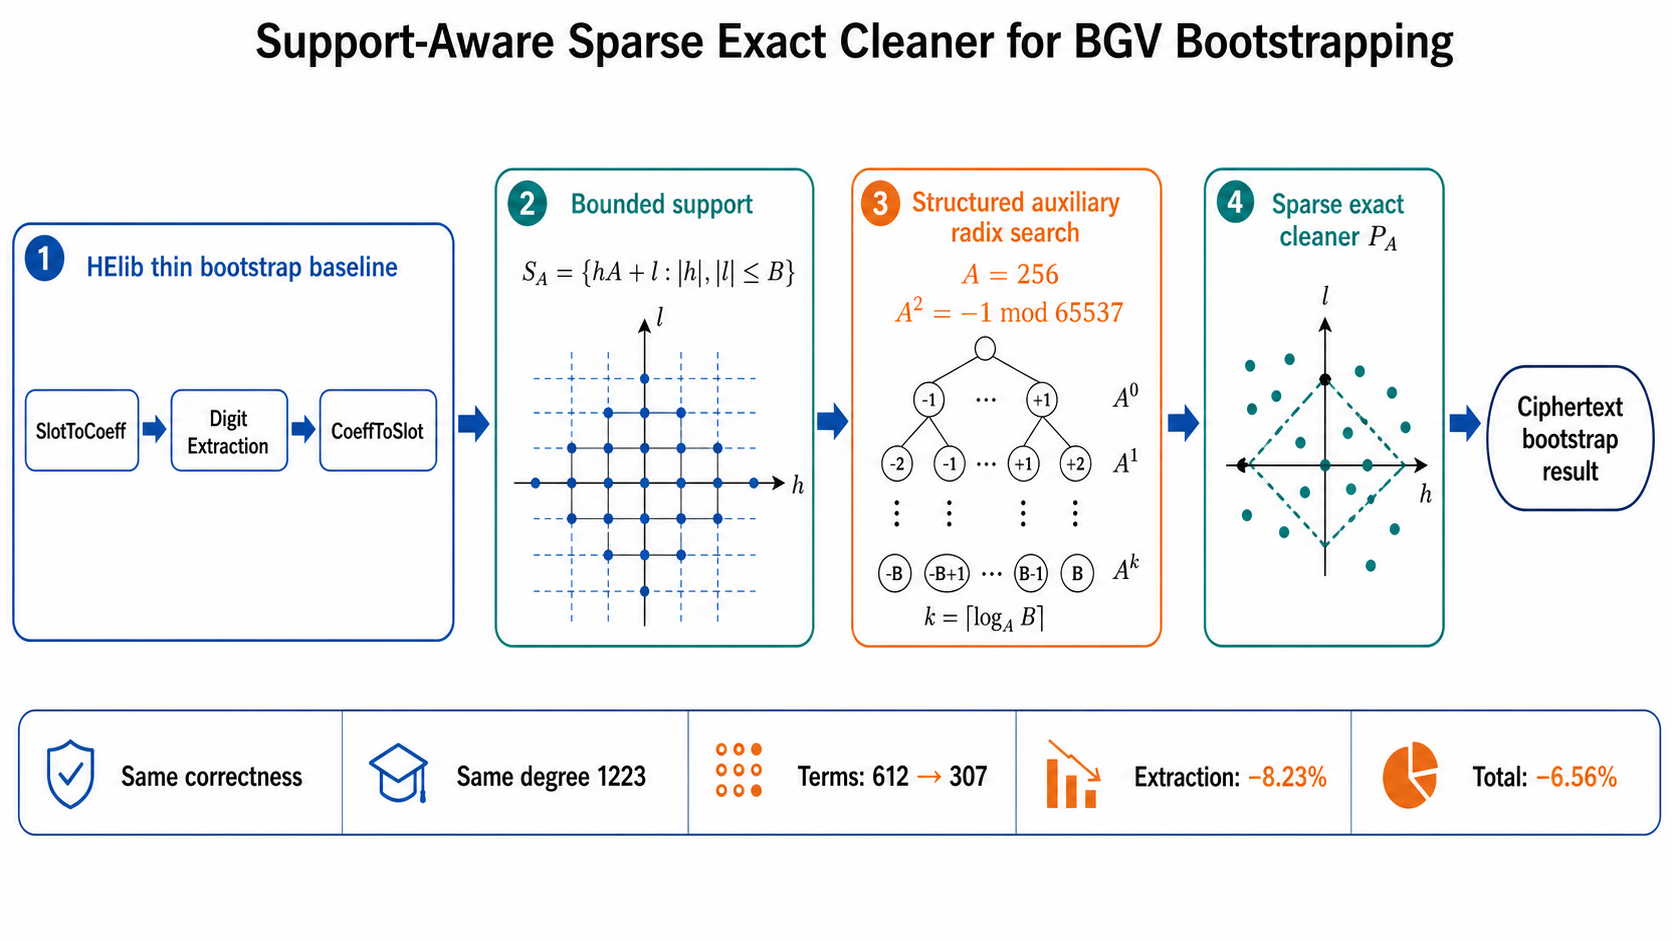
\includegraphics[width=\linewidth]{figures/image2_overview.png}
}{%
\resizebox{\linewidth}{!}{%
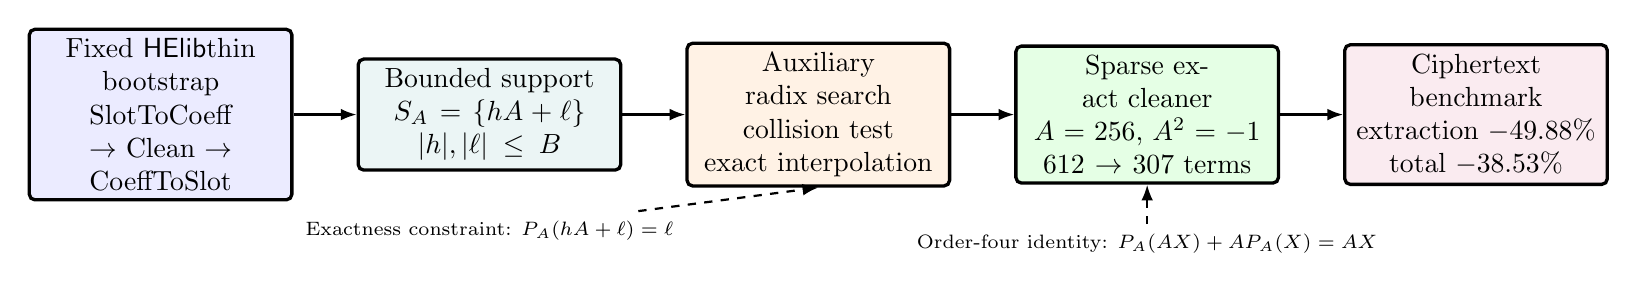
\begin{tikzpicture}[
  node distance=8mm,
  box/.style={draw, rounded corners=2pt, very thick, align=center,
    minimum height=10mm, text width=31mm, fill=white},
  small/.style={font=\scriptsize, align=center},
  arr/.style={-{Latex[length=2mm]}, thick}
]
  \node[box, fill=blue!8] (base) {Fixed \HElib thin bootstrap\\
    SlotToCoeff $\rightarrow$ Clean $\rightarrow$ CoeffToSlot};
  \node[box, fill=teal!8, right=of base] (support) {Bounded support\\
    $S_A=\{hA+\ell\}$\\$|h|,|\ell|\le B$};
  \node[box, fill=orange!10, right=of support] (search) {Auxiliary radix search\\
    collision test\\exact interpolation};
  \node[box, fill=green!10, right=of search] (cleaner) {Sparse exact cleaner\\
    $A=256$, $A^2=-1$\\$612\rightarrow307$ terms};
  \node[box, fill=purple!8, right=of cleaner] (bench) {Ciphertext benchmark\\
    extraction $-49.88\%$\\total $-38.53\%$};
  \draw[arr] (base) -- (support);
  \draw[arr] (support) -- (search);
  \draw[arr] (search) -- (cleaner);
  \draw[arr] (cleaner) -- (bench);
  \node[small, below=5mm of support] (eq1)
    {Exactness constraint: $P_A(hA+\ell)=\ell$};
  \node[small, below=5mm of cleaner] (eq2)
    {Order-four identity: $P_A(AX)+AP_A(X)=AX$};
  \draw[arr, dashed] (eq1) -- (search.south);
  \draw[arr, dashed] (eq2) -- (cleaner.south);
\end{tikzpicture}}}
\caption{Overview of the support-aware sparse-cleaner route.  If the
Image-2 rendering is present in \texttt{figures/image2\_overview.png}, it is
used; otherwise the paper compiles with this TikZ fallback.  Numeric claims
are backed by Tables~\ref{tab:term_structure} and~\ref{tab:helib_repeat3}.}
\label{fig:overview}
\end{figure}

\subsection{What Changes and What Does Not}

The optimization changes only the exact cleaner representative used in the
digit-extraction step.  It does not change the plaintext modulus, cyclotomic
index, secret-key distribution, linear-transform keys, or ciphertext
correctness criterion.

\begin{table}[t]
\centering
\caption{Design invariants and modified components.}
\label{tab:design_invariants}
\begin{tabular}{p{3.5cm}p{4.3cm}p{4.0cm}}
\toprule
\textbf{Component} & \textbf{Baseline} & \textbf{This work} \\
\midrule
Plaintext modulus & $p=65537$ & unchanged \\
Bound parameter & $B=17$ & unchanged \\
Support size & $(2B+1)^2=1225$ & unchanged \\
Auxiliary radix & generic $A=35$ & structured $A=256$ \\
Cleaner degree & $1223$ & $1223$ \\
Cleaner terms & $612$ & $307$ \\
Linear maps & \HElib BSGS/hoisting & unchanged in main claim \\
Correctness test & \HElib success marker & unchanged; all main runs pass \\
\bottomrule
\end{tabular}
\end{table}

\subsection{Running Example}

For $p=65537$ and $B=17$, the support contains $35^2=1225$ points if
$(h,\ell)\mapsto hA+\ell$ is injective on the square.  The generic baseline
radix $A=35$ gives a canonical cleaner of degree $1223$ with $612$ nonzero
monomials.  The order-four radix $A=256$ also gives degree $1223$ but only
$307$ nonzero monomials.  This example captures the paper's central
distinction:
\[
  \text{degree reduction}\quad \neq \quad
  \text{sparse representative selection}.
\]
The first is already provided by the bounded-support null-polynomial
framework.  The second is the new optimization studied here.

% ================================================================
\section{Support-Aware Exact Cleaner Theory}
\label{sec:theory}
% ================================================================

\subsection{Bounded Supports}

Let $p$ be an odd prime and let $A\in\Fp^\times$.  For a bound $B\ge 1$,
define the square-indexed support
\[
  S_A=\{hA+\ell \bmod p: h,\ell\in[-B,B]\}\subseteq\Fp .
\]
We say $A$ is \emph{$B$-injective} if the map
\[
  \phi_A:[-B,B]^2\to\Fp,\qquad (h,\ell)\mapsto hA+\ell
\]
is injective.  In the target setting $B=17$, both $A=35$ and $A=256$ are
$B$-injective.  When injectivity holds, the exact cleaner is the support
function
\[
  C_A:S_A\to\Fp,\qquad C_A(hA+\ell)=\ell.
\]
The role of $C_A$ in bootstrapping is to recover the bounded low coordinate
from a noisy residue encoded by the auxiliary radix.

\subsection{The Support Quotient}

Let
\[
  G_{S_A}(X)=\prod_{s\in S_A}(X-s).
\]
The polynomial $G_{S_A}$ is the support vanishing polynomial.  All exact
cleaners are representatives of the same coset modulo $(G_{S_A})$.

\begin{lemma}[Support quotient]
\label{lem:support_quotient}
Let $S\subset\Fp$ be finite and let $G_S(X)=\prod_{s\in S}(X-s)$.  For
$F,Q\in\Fp[X]$, the following are equivalent:
\[
  F(s)=Q(s)\quad\text{for every }s\in S,
  \qquad
  F-Q\in(G_S).
\]
Consequently, each function $S\to\Fp$ has a unique representative of degree
$<|S|$.
\end{lemma}

\begin{proof}
If $F-Q$ is divisible by $G_S$, it vanishes on $S$.  Conversely, if $F-Q$
vanishes on $S$, then every $X-s$ with $s\in S$ divides $F-Q$.  The roots are
distinct in the field $\Fp$, so their product $G_S$ divides $F-Q$.  Euclidean
division by $G_S$ gives a unique remainder of degree $<|S|$.
\end{proof}

\begin{definition}[Canonical exact cleaner]
For a $B$-injective radix $A$, $P_A$ denotes the unique degree-$<|S_A|$
polynomial in $\Fp[X]$ satisfying
\[
  P_A(hA+\ell)=\ell\qquad\text{for all }h,\ell\in[-B,B].
\]
\end{definition}

\subsection{Degree-Minimality}

The canonical representative gives a simple but important certificate.  If it
has degree $d$, then a lower-degree exact univariate cleaner on the same
support does not exist.

\begin{lemma}[Fixed-support degree certificate]
\label{lem:degree_certificate}
Let $P_A$ be the canonical exact cleaner on an injective support $S_A$ and
let $\deg(P_A)=d$.  No exact univariate cleaner for $C_A$ on $S_A$ has degree
strictly below $d$.
\end{lemma}

\begin{proof}
Suppose $Q$ is exact on $S_A$ and $\deg(Q)<d$.  By
Lemma~\ref{lem:support_quotient}, $P_A-Q$ is divisible by $G_{S_A}$.  But
both $P_A$ and $Q$ have degree below $|S_A|$, so $P_A-Q$ has degree below
$|S_A|$.  The only multiple of $G_{S_A}$ with degree below $|S_A|$ is zero.
Hence $P_A=Q$, contradicting $\deg(Q)<\deg(P_A)$.
\end{proof}

This lemma is the reason the paper is careful about its claim.  For
$p=65537$, $B=17$, both $A=35$ and $A=256$ have degree $1223$, and that degree
is minimal for their respective supports.  The improvement is not a lower
degree for the same support.  It is a sparser representative induced by a
better support geometry.

\subsection{Interpolation Formula}

For completeness, the canonical cleaner can be written by Lagrange
interpolation:
\[
  P_A(X)=\sum_{h=-B}^B\sum_{\ell=-B}^B
  \ell\cdot
  \prod_{\substack{(h',\ell')\in[-B,B]^2\\(h',\ell')\ne(h,\ell)}}
  \frac{X-(h'A+\ell')}{(hA+\ell)-(h'A+\ell')}.
\]
This formula is not the evaluation method used in \HElib.  It is a synthesis
definition: after interpolation, the polynomial is reduced to its nonzero
monomial coefficients and evaluated by the library's polynomial evaluator.

\subsection{Evaluation-Aware Objectives}

The encrypted cost of evaluating a polynomial is not determined by degree
alone.  Let
\[
  P(X)=\sum_{k\in T} c_kX^k
\]
with term set $T$.  A Paterson--Stockmeyer style evaluator first builds baby
powers, then giant powers, then accumulates nonzero coefficient blocks.  A
rough implementation-level proxy is
\[
  C_{\mathrm{eval}}(P)
  =
  C_{\mathrm{pow}}(\deg P)
  + C_{\mathrm{acc}}(|T|,\operatorname{block}(T))
  + C_{\mathrm{scalar}}(|T|).
\]
The first term is mainly controlled by degree.  The second and third terms are
affected by sparsity and by how nonzero exponents distribute across blocks.
Therefore, a $49.84\%$ reduction in term count should not be expected to give
a $49.84\%$ ciphertext speedup.  It can still reduce scalar multiplies,
accumulations, memory traffic, and some evaluator overhead, which is exactly
what the \HElib timing shows.

\begin{table}[t]
\centering
\caption{Optimization objectives after bounded-support degree reduction.}
\label{tab:objective}
\begin{tabular}{p{3.0cm}p{4.5cm}p{4.2cm}}
\toprule
\textbf{Objective} & \textbf{What it measures} & \textbf{Status here} \\
\midrule
Exactness & $P_A(hA+\ell)=\ell$ for all support points & fully verified \\
Fixed-support degree & minimum possible degree for chosen $S_A$ & certified, degree $1223$ \\
Monomial sparsity & number of nonzero coefficients & $612\rightarrow307$ \\
Evaluation cost & \HElib encrypted polynomial-evaluation time & extraction $49.88\%$ faster \\
Pipeline correctness & full ciphertext bootstrap output & all main repeat-three runs pass \\
\bottomrule
\end{tabular}
\end{table}

% ================================================================
\section{Order-Four Radix Structure}
\label{sec:order4}
% ================================================================

\subsection{Quarter-Turn Symmetry}

Assume $A^2=-1\bmod p$.  Then multiplication by $A$ has order four in
$\Fp^\times$.  On the support coordinates, it acts as
\[
  A(hA+\ell)=hA^2+\ell A=\ell A-h,
\]
which corresponds to the quarter-turn
\[
  (h,\ell)\mapsto(\ell,-h).
\]
Since the square $[-B,B]^2$ is stable under this map, $S_A$ is stable under
multiplication by $A$.

\begin{figure}[t]
\centering
\IfFileExists{figures/image2_structure.png}{%
  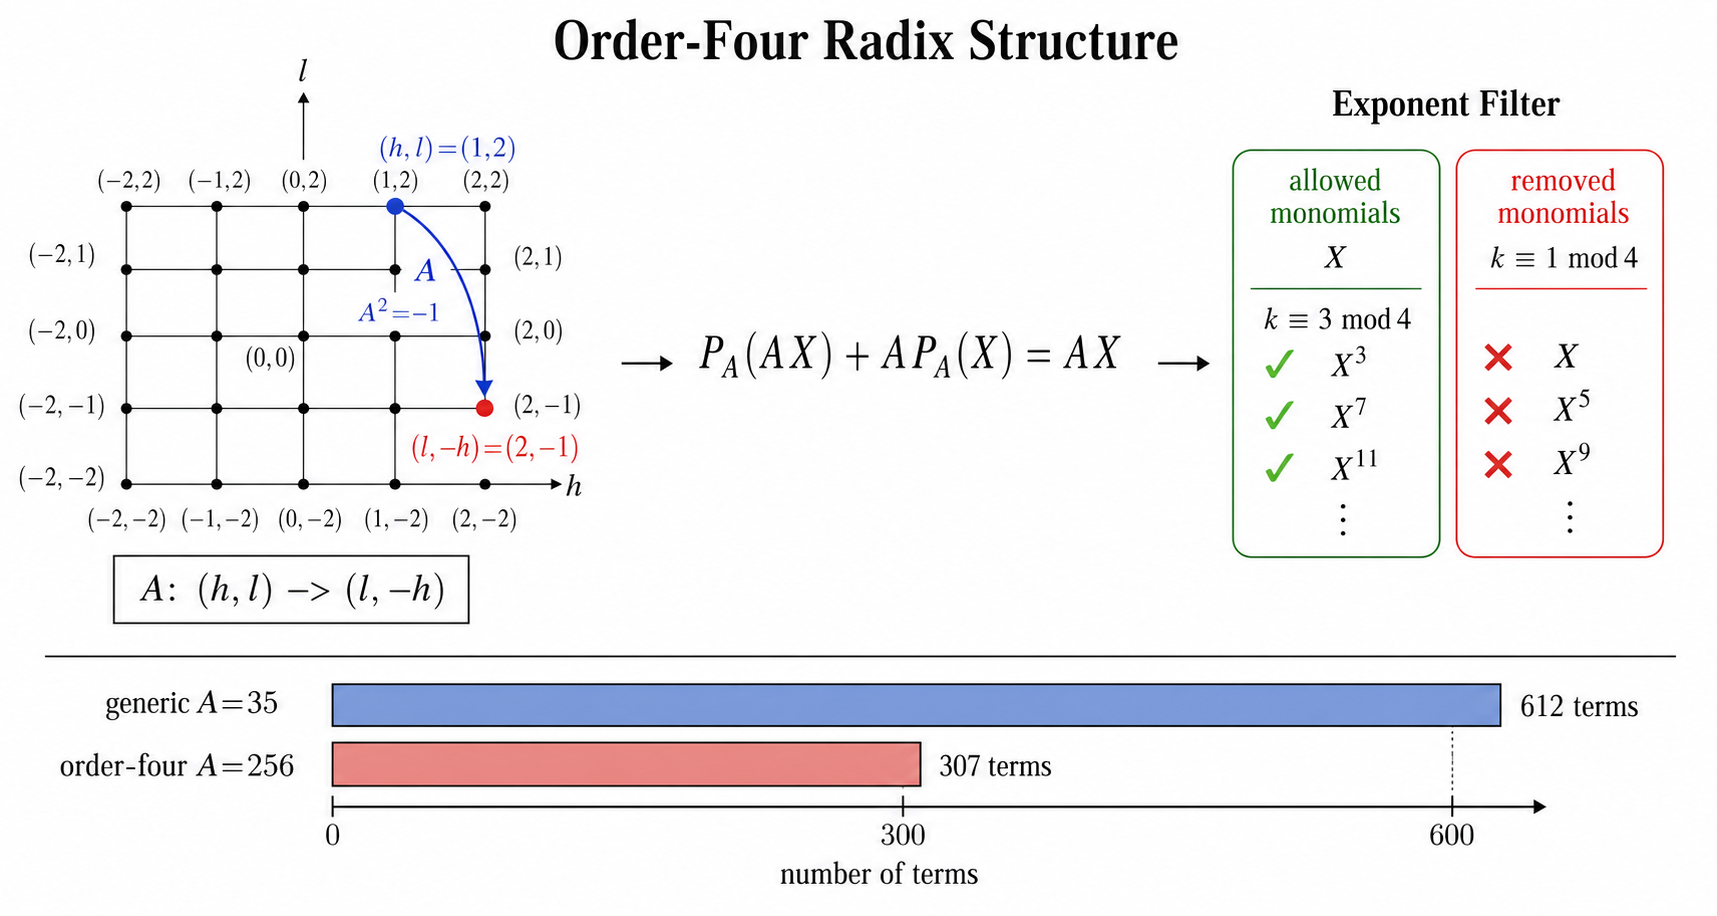
\includegraphics[width=\linewidth]{figures/image2_structure.png}
}{%
\resizebox{\linewidth}{!}{%
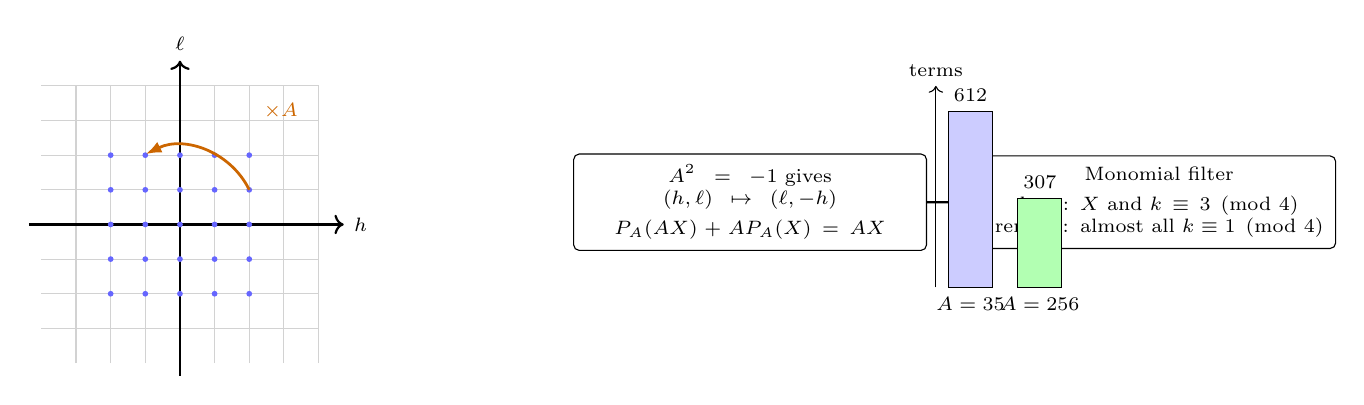
\begin{tikzpicture}[
  scale=0.8,
  every node/.style={font=\scriptsize},
  arr/.style={-{Latex[length=2mm]}, thick},
  box/.style={draw, rounded corners=2pt, align=center, fill=white, inner sep=4pt}
]
  \draw[step=0.55cm, gray!35] (-2.2,-2.2) grid (2.2,2.2);
  \draw[->, thick] (-2.4,0) -- (2.6,0) node[right] {$h$};
  \draw[->, thick] (0,-2.4) -- (0,2.6) node[above] {$\ell$};
  \foreach \x in {-2,-1,0,1,2}
    \foreach \y in {-2,-1,0,1,2}
      \fill[blue!60] (0.55*\x,0.55*\y) circle (1.3pt);
  \draw[arr, orange!80!black, line width=1pt] (1.1,0.55) arc[start angle=26,end angle=116,radius=1.23];
  \node[orange!80!black] at (1.6,1.8) {$\times A$};
  \node[box, right=25mm of current bounding box.east, text width=42mm] (eq)
    {$A^2=-1$ gives\\$(h,\ell)\mapsto(\ell,-h)$\\[1mm]
     $P_A(AX)+AP_A(X)=AX$};
  \node[box, right=7mm of eq, text width=42mm] (filter)
    {Monomial filter\\[1mm]
     keep: $X$ and $k\equiv3\pmod4$\\
     remove: almost all $k\equiv1\pmod4$};
  \draw[arr] (eq) -- (filter);
  \begin{scope}[xshift=12.2cm,yshift=-1.0cm]
    \draw[fill=blue!20] (0,0) rectangle (0.7,2.8);
    \draw[fill=green!30] (1.1,0) rectangle (1.8,1.41);
    \node[below] at (0.35,0) {$A=35$};
    \node[below] at (1.45,0) {$A=256$};
    \node[above] at (0.35,2.8) {$612$};
    \node[above] at (1.45,1.41) {$307$};
    \draw[->] (-0.2,0) -- (-0.2,3.2) node[above] {terms};
  \end{scope}
\end{tikzpicture}}}
\caption{Order-four radix structure.  Multiplication by $A$ rotates the
support square, and the cleaner's covariance under that rotation filters the
monomial support.}
\label{fig:order_four}
\end{figure}

\subsection{Functional Identity}

\begin{theorem}[Order-four sparsity]
\label{thm:order_four}
Let $A^2=-1\bmod p$ and assume $A$ is $B$-injective.  Let $P_A$ be the
canonical exact cleaner on $S_A$.  Then
\[
  P_A(AX)+A P_A(X)=AX.
\]
If $P_A(X)=\sum_k c_kX^k$, then $c_k=0$ for all
$k\not\equiv 3\pmod 4$ except possibly $k=1$, and $c_1=1/2$.
\end{theorem}

\begin{proof}
Take a support point $x=hA+\ell$.  By definition, $P_A(x)=\ell$.  Since
$Ax=\ell A-h$, the cleaner value at $Ax$ is $P_A(Ax)=-h$.  Also
\[
  A(x-P_A(x))=A(hA+\ell-\ell)=AhA=-h.
\]
Hence
\[
  P_A(Ax)+A P_A(x)-Ax=0
\]
for every $x\in S_A$.  The left-hand side has degree below $|S_A|$ because
$P_A$ does.  It vanishes on $|S_A|$ distinct points, so it is the zero
polynomial by Lemma~\ref{lem:support_quotient}.

Now write $P_A(X)=\sum_k c_kX^k$.  The identity gives
\[
  \sum_k c_k(A^k+A)X^k-AX=0.
\]
For $k\ne1$, a nonzero $c_k$ requires $A^k+A=0$, i.e.,
$A^{k-1}=-1=A^2$.  Since $A$ has order four, this is equivalent to
$k\equiv3\pmod4$.  For $k=1$, the coefficient equation is
$(A+A)c_1=A$, so $c_1=1/2$ in $\Fp$.
\end{proof}

\subsection{Character-Space Interpretation}

The proof can be phrased in the language of finite-field representations.
Let $T_A$ be the linear operator on $\Fp[X]/(G_{S_A})$ defined by
\[
  (T_AF)(X)=F(AX).
\]
When $A^2=-1$, $T_A^4=1$ on the support quotient.  The monomial $X^k$ is an
eigenvector of the substitution operator with eigenvalue $A^k$, up to the
degree-$<|S_A|$ representative.  The homogeneous part of the cleaner identity
selects the eigenspace with eigenvalue $-A=A^3$.  This is why the allowed
exponents satisfy $k\equiv3\pmod4$.  The inhomogeneous term $AX$ forces the
single linear monomial with coefficient $1/2$.

This viewpoint is useful because it suggests a general design rule:
look for auxiliary radices whose action on the bounded support is a small
group action, then synthesize the cleaner in the corresponding character
subspaces.  The present paper implements the most stable case, the order-four
rotation, because it is easy to certify and it is compatible with the target
prime $65537$.


\subsection{Order-Adaptive Higher-Order Generalization}

The order-four theorem is the first nontrivial instance of a broader subgroup
principle.  Let $U=\langle A\rangle\subset\Fp^\times$ be a finite cyclic
subgroup of order $r$, and suppose the bounded support model is chosen so that
multiplication by $A$ acts as a signed permutation on a small coordinate tuple.
Then the canonical cleaner can be projected into character subspaces of the
substitution operator $T_A:F(X)\mapsto F(AX)$ on the support quotient.  In
favorable cases, this removes most monomial residue classes before any
homomorphic evaluation is performed.

For the current paper we keep this generalization conservative.  We do not
claim a full higher-order ciphertext implementation.  Instead, we use it as a
planner for deciding when the order-four implemented route is already optimal
and when a higher-order route could become attractive on a smaller local
support.

The cleanest dyadic model is the signed-circulant representation.  For an order
$r=2d$ candidate, write
\[
  x = u_0 + u_1A + \cdots + u_{d-1}A^{d-1},
\]
with bounded integer coordinates $u_j\in[-B,B]$ and relation $A^d=-1$.
Multiplication by $A$ then acts as a signed cyclic shift:
\[
  A(u_0,\ldots,u_{d-1}) = (-u_{d-1},u_0,\ldots,u_{d-2}).
\]
A sufficient collision-free condition for this representation is
\[
  (2B+1)\sum_{j=0}^{d-1}|A|^j < p.
\]
This bound is not necessary, but it is simple, exact, and adequate for the
paper's planner role.

For $p=65537$, the dyadic tower in $\Fp^\times$ is particularly explicit:
\[
  256^2=-1,\qquad 16^4=-1,\qquad 4^8=-1,\qquad 2^{16}=-1.
\]
Thus the natural dyadic candidates are:
\[
  (r,A,d)=(4,256,2),\ (8,16,4),\ (16,4,8),\ (32,2,16).
\]
Applying the sufficient bound gives immediate global thresholds:
\[
  r=4: B\le 127,
  \qquad
  r=8: B\le 7,
  \qquad
  r=16: B\le 1.
\]
The order-$32$ candidate is too restrictive to be useful in the present large-$p$
setting.  These thresholds match the offline exact interpolation sweep in
Section~\ref{sec:search}: for the implemented global support radius $B=17$,
order four is the only stable dyadic choice; order eight first becomes
support-safe at smaller local radii such as $B\le 7$; and order sixteen is
reserved for tiny local supports.
This yields the paper's conservative planner rule:
\begin{quote}
Use the implemented order-four cleaner as the global large-support route, and
only consider higher subgroup order after an earlier transform or local support
argument has already compressed the effective radius enough to satisfy the
corresponding signed-circulant bound.
\end{quote}

The role of this rule is twofold.  First, it prevents a misleading “higher order
is always better” narrative.  Second, it connects the nonlinear cleaner design
to the linear-transform side: support shaping can unlock cleaner orders that are
impossible in the original global support.

\begin{table}[t]
\centering
\caption{Monomial support structure for the target parameter set
$p=65537$, $B=17$.}
\label{tab:term_structure}
\begin{tabular}{rrrrr}
\toprule
\textbf{Radix $A$} & \textbf{Type} & \textbf{Degree} &
\textbf{Terms} & \textbf{Nonzero exponent classes} \\
\midrule
$35$ & generic & $1223$ & $612$ &
$306$ in $1\bmod4$, $306$ in $3\bmod4$ \\
$256$ & $A^2=-1$ & $1223$ & $307$ &
$1$ in $1\bmod4$, $306$ in $3\bmod4$ \\
\bottomrule
\end{tabular}
\end{table}

% ================================================================
\section{SAT and Structured Search}
\label{sec:search}
% ================================================================

We use two search modes.  In the small setting $p=257$, $B=5$, we enumerate
all nonzero radices and therefore get a complete global search over the radix
domain.  In the target setting $p=65537$, $B=17$, complete enumeration is
unnecessary for the paper's claim; instead we use a structured candidate set
containing explicit baselines, low-order elements, and roots of small
algebraic equations such as $X^2+1=0$.

\begin{figure}[t]
\centering
\IfFileExists{figures/image2_sat_search.png}{%
  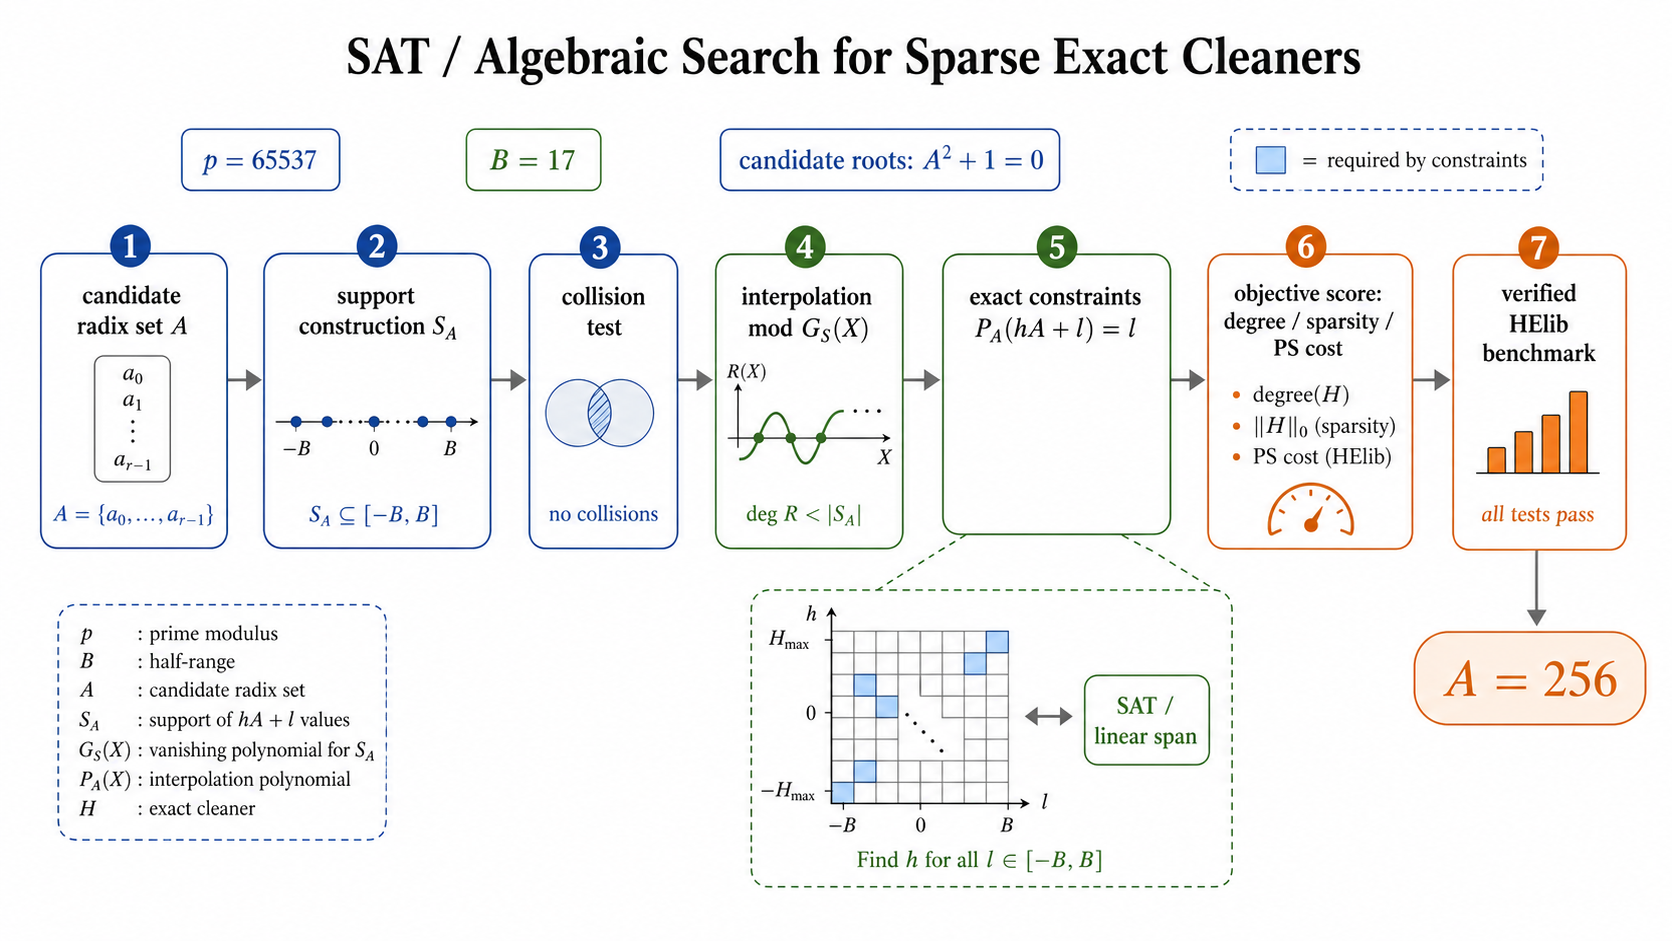
\includegraphics[width=\linewidth]{figures/image2_sat_search.png}
}{%
\resizebox{\linewidth}{!}{%
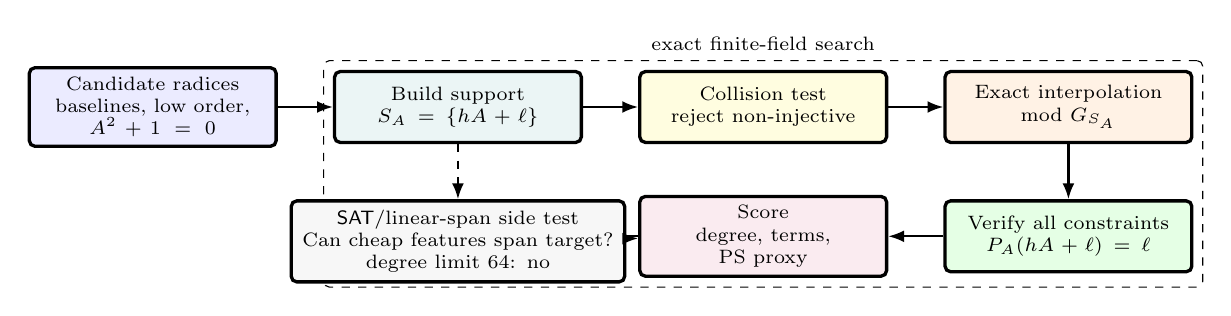
\begin{tikzpicture}[
  node distance=7mm,
  box/.style={draw, rounded corners=2pt, very thick, align=center,
    minimum height=9mm, text width=29mm, fill=white},
  arr/.style={-{Latex[length=2mm]}, thick},
  every node/.style={font=\scriptsize}
]
  \node[box, fill=blue!8] (cand) {Candidate radices\\baselines, low order,\\$A^2+1=0$};
  \node[box, fill=teal!8, right=of cand] (support) {Build support\\$S_A=\{hA+\ell\}$};
  \node[box, fill=yellow!12, right=of support] (collision) {Collision test\\reject non-injective};
  \node[box, fill=orange!10, right=of collision] (interp) {Exact interpolation\\mod $G_{S_A}$};
  \node[box, fill=green!10, below=of interp] (verify) {Verify all constraints\\$P_A(hA+\ell)=\ell$};
  \node[box, fill=purple!8, left=of verify] (score) {Score\\degree, terms,\\PS proxy};
  \node[box, fill=red!7, left=of score] (bench) {HElib benchmark\\selected candidates};
  \draw[arr] (cand) -- (support);
  \draw[arr] (support) -- (collision);
  \draw[arr] (collision) -- (interp);
  \draw[arr] (interp) -- (verify);
  \draw[arr] (verify) -- (score);
  \draw[arr] (score) -- (bench);
  \node[draw, dashed, rounded corners=2pt, fit=(support)(collision)(interp)(verify)(score),
    label={[font=\scriptsize]above:exact finite-field search}] {};
  \node[box, fill=gray!6, below=of support, text width=40mm] (sat)
    {\Sat/linear-span side test\\Can cheap features span target?\\degree limit $64$: no};
  \draw[arr, dashed] (support) -- (sat);
  \draw[arr, dashed] (sat) -- (score);
\end{tikzpicture}}}
\caption{Structured search and \Sat/linear-span side test.  The exact
interpolation path is the main synthesis route; the bounded feature search is
used to test whether an even cheaper low-degree feature library spans the
target function.}
\label{fig:sat_search}
\end{figure}

\subsection{Exact Synthesis Algorithm}

\begin{algorithm}[t]
\caption{Support-aware exact cleaner synthesis}
\label{alg:synthesis}
\begin{algorithmic}[1]
\Require prime $p$, bound $B$, candidate radix set $\mathcal{A}$
\Ensure ranked exact cleaners
\State $R\gets []$
\ForAll{$A\in\mathcal{A}$}
  \State $S\gets []$, $\mathsf{values}\gets []$, $\mathsf{collision}\gets\textbf{false}$
  \For{$h=-B$ to $B$}
    \For{$\ell=-B$ to $B$}
      \State $s\gets hA+\ell\bmod p$
      \If{$s\in S$} \State $\mathsf{collision}\gets\textbf{true}$ \EndIf
      \State append $s$ to $S$ and $\ell\bmod p$ to $\mathsf{values}$
    \EndFor
  \EndFor
  \If{$\mathsf{collision}$} \State \textbf{continue} \EndIf
  \State interpolate $P_A\in\Fp[X]$ with $P_A(S_i)=\mathsf{values}_i$
  \State verify $P_A(hA+\ell)=\ell$ for all $h,\ell\in[-B,B]$
  \State compute degree, term count, residue-class histogram, evaluation proxy
  \State append $(A,P_A,\mathsf{score})$ to $R$
\EndFor
\State \Return $R$ sorted by exactness, degree, term count, and proxy cost
\end{algorithmic}
\end{algorithm}

All arithmetic in Algorithm~\ref{alg:synthesis} is over $\Fp$.  The output is
not accepted unless exact verification succeeds on every support point.

\subsection{SAT and Feature-Span View}

The word \Sat is used in this project in a precise experimental sense.  We
consider a finite feature library
\[
  \mathcal{F}=\{f_1(X),\ldots,f_m(X)\}
\]
and ask whether the target cleaner lies in its span on $S_A$:
\[
  C_A(s)=\sum_{i=1}^m \alpha_i f_i(s)
  \qquad\text{for all }s\in S_A.
\]
Over $\Fp$, the span test is a linear algebra problem.  If one additionally
asks for a minimum number of selected features, the problem becomes an
$\ell_0$ selection problem that can be encoded as a Boolean or SMT search.
The current artifact includes a degree-limited mixed-feature side test for
$A=256$; with degree limit $64$ and $160$ features, the target is not in the
span.  This negative result helps rule out an overly optimistic claim that a
very low-degree cheap feature library already suffices.

\subsection{Search Results}

\begin{table}[t]
\centering
\caption{Exact cleaner search results.  The small-field row is a complete
search over all nonzero radices; the target row is a structured algebraic
search.}
\label{tab:search_results}
\begin{tabular}{rrrrrll}
\toprule
$p$ & $B$ & candidates & valid & best $A$ & degree & terms \\
\midrule
$257$ & $5$ & $255$ & $130$ & $16,241$ & $119$ & $31$ \\
$65537$ & $17$ & $65$ & $44$ & $256,65281$ & $1223$ & $307$ \\
\bottomrule
\end{tabular}
\end{table}

\begin{table}[t]
\centering
\caption{Degree certificates for generic and order-four radices.}
\label{tab:degree_certificates}
\begin{tabular}{lrrrrr}
\toprule
$p$ & $B$ & $A$ & support size & degree & terms \\
\midrule
$257$ & $5$ & $35$ & $121$ & $119$ & $60$ \\
$257$ & $5$ & $16$ & $121$ & $119$ & $31$ \\
$65537$ & $17$ & $35$ & $1225$ & $1223$ & $612$ \\
$65537$ & $17$ & $256$ & $1225$ & $1223$ & $307$ \\
\bottomrule
\end{tabular}
\end{table}

\begin{table}[t]
\centering
\caption{Order-adaptive planner sweep for $p=65537$.  The positive ciphertext
claim is only the implemented order-four row at $B=17$; the higher-order rows
are offline exact-search and threshold evidence.}
\label{tab:order_adaptive_sweep}
\scriptsize
\begin{tabular}{rrrrllp{4.7cm}}
\toprule
$B$ & support & degree & terms & best decomposition & dyadic-safe orders & planner recommendation \\
\midrule
$1$  & $9$    & $7$    & $3$   & mod-$2$, est. $4$ mults  & $4,8,16$ & order-$16$ is support-safe but only as a tiny-local-support theory target \\
$3$  & $49$   & $47$   & $13$  & mod-$4$, est. $10$ mults & $4,8$    & first range where order-$8$ becomes support-safe \\
$5$  & $121$  & $119$  & $31$  & mod-$4$, est. $15$ mults & $4,8$    & order-$8$ remains plausible on smaller local supports \\
$7$  & $225$  & $223$  & $57$  & mod-$4$, est. $19$ mults & $4,8$    & largest tested radius where order-$8$ stays support-safe \\
$9$  & $361$  & $359$  & $91$  & mod-$4$, est. $24$ mults & $4$      & higher dyadic orders no longer satisfy the sufficient bound \\
$17$ & $1225$ & $1223$ & $307$ & mod-$4$, est. $41$ mults & $4$      & implemented global case; order-$4$ is the stable choice \\
\bottomrule
\end{tabular}
\end{table}

The small complete search is useful because it eliminates candidate-selection
bias at a manageable scale.  It selects the two roots of $-1$ modulo $257$,
$16$ and $241$, as the best radices by term count.  The target structured
search similarly selects $256$ and $65281=-256\bmod65537$.  The practical
\HElib radix is the small positive representative $256$ because the integer
radix also affects mod-up and overflow scaling in the implementation.

The new order-adaptive sweep adds an important claim boundary.  For the target
prime $65537$, the implemented global support radius $B=17$ is already too large
for the order-$8$ signed-circulant sufficient bound, so the paper should not
suggest that “higher subgroup order” is immediately available inside the same
pipeline.  Conversely, the rows $B\in\{3,5,7\}$ show that order eight becomes a
real planner target once an earlier local argument or support-shaping transform
compresses the effective radius enough.  This is the sense in which the paper's
higher-order cleaner story is conservative but nontrivial: it is grounded in
exact interpolation and threshold data, not just algebraic speculation.


% ================================================================
\section{Implementation}
\label{sec:implementation}
% ================================================================

\subsection{Artifact Layout}

All implementation work for this paper is placed in the isolated upload
directory of the project, so the baseline code collection is not polluted.
The paper directory contains only the manuscript, references, and figures.
The main artifact files are listed in
Table~\ref{tab:artifact_layout}.

\begin{table}[t]
\centering
\caption{Artifact components used by the paper.}
\label{tab:artifact_layout}
\scriptsize
\begin{tabular}{p{4.6cm}p{7.1cm}}
\toprule
\textbf{Path} & \textbf{Role} \\
\midrule
\path{scripts/aux_cleaning_global_sweep.py}
& complete small-field radix sweep and exact interpolation \\
\path{scripts/structured_aux_cleaner_experiment.py}
& structured algebraic target search \\
\path{scripts/cleaner_degree_certificate.py}
& fixed-support degree-minimality certificate \\
\path{scripts/cleaner_term_structure.py}
& monomial residue-class analysis \\
\path{scripts/sat_cleaning_circuit_search.py}
& \Sat/linear-span feature search \\
\path{scripts/parse_helib_bootstrap_timings.py}
& parser for \HElib repeat logs \\
\path{results/paper_routes/*.json}
& exact search, degree, and timing outputs \\
\path{results/upload_aux_default_repeat3.log}
& baseline ciphertext bootstrapping log \\
\path{results/upload_aux_256_repeat3.log}
& sparse-cleaner ciphertext bootstrapping log \\
\bottomrule
\end{tabular}
\end{table}

\subsection{HElib Integration}

The \HElib integration adds an explicit auxiliary-radix option to the isolated
upload copy of the code.  The default run uses the baseline radix.  Setting
\[
  \texttt{HELIB\_EXPLICIT\_AUX=256}
\]
selects the order-four radix.  The bootstrapping driver then constructs the
corresponding exact cleaner and evaluates it in the existing digit-extraction
stage.  The surrounding pipeline remains fixed:
\[
  \text{linear transform 1}
  \;\rightarrow\;
  \text{sparse exact extraction}
  \;\rightarrow\;
  \text{linear transform 2}.
\]

\subsection{Parameter Set}

The real ciphertext benchmark uses the \HElib large-prime thin-bootstrapping
setting
\[
  p=65537,\qquad B=17,\qquad m=50731,\qquad
  \mathrm{mvec}=[97,523],\qquad \mathrm{ords}=[96,29].
\]
The support size is $(2B+1)^2=1225$.  The comparison is between:
\[
  A=35\quad\text{(generic baseline)},\qquad
  A=256\quad\text{(order-four sparse cleaner)}.
\]

\subsection{Correctness Criterion}

Each ciphertext benchmark must finish with the \HElib success marker
\[
  \texttt{\#\#\# bts finished, everything ok \#\#\#}.
\]
All main $A=35$ and $A=256$ repeat-three runs satisfy this criterion.  Failed
linear-transform fusion attempts are explicitly separated in
Section~\ref{sec:linear-negative}.

% ================================================================
\section{Evaluation}
\label{sec:evaluation}
% ================================================================

\subsection{Experimental Questions}

The evaluation answers five questions:
\begin{enumerate}[leftmargin=*]
  \item Does structured search find a cleaner with lower monomial support than
  the generic baseline?
  \item Is the degree still minimal, making the implemented claim a sparsity
  and evaluation-cost claim rather than an invalid lower-degree claim?
  \item Do the order-four cleaner and its specialized evaluator improve real
  ciphertext bootstrapping time?
  \item What does the order-adaptive sweep say about when higher subgroup order
  is actually support-safe for $p=65537$?
  \item Do the current linear-transform experiments justify a second positive
  ciphertext claim, or only a design/planner claim with explicit boundaries?
\end{enumerate}

\subsection{Ciphertext Timing Results}

Table~\ref{tab:helib_repeat3} reports the main repeat-three benchmark.  The
numbers are wall-clock seconds parsed from the raw \HElib logs.  The two runs
use the same artifact, parameter set, and correctness condition.

\begin{table}[t]
\centering
\caption{\HElib thin-bootstrapping benchmark, repeat-three mean.}
\label{tab:helib_repeat3}
\begin{tabular}{rlrrrr}
\toprule
\textbf{Radix $A$} & \textbf{terms} & \textbf{linear1} &
\textbf{linear2} & \textbf{extract} & \textbf{total} \\
\midrule
$35$ & $612$ & $4.400641$s & $45.190252$s &
$161.168362$s & $213.389347$s \\
$256$ & $307$ & $4.380695$s & $44.512004$s &
$147.909934$s & $199.397017$s \\
$256$ + order-four eval & $307$ & $4.272161$s & $43.623283$s &
$80.770389$s & $131.180978$s \\
\midrule
Sparse improvement & $49.84\%$ fewer & $0.45\%$ & $1.50\%$ &
$8.23\%$ & $6.56\%$ \\
Full improvement & $49.84\%$ fewer & $2.92\%$ & $3.47\%$ &
$49.88\%$ & $38.53\%$ \\
\bottomrule
\end{tabular}
\end{table}

\begin{table}[t]
\centering
\caption{Per-run repeat-three timings.}
\label{tab:per_run}
\scriptsize
\begin{tabular}{rrrrrr}
\toprule
\textbf{run} & \textbf{$A$} & \textbf{linear1} & \textbf{linear2} &
\textbf{extract} & \textbf{total} \\
\midrule
1 & $35$ & $4.561208$s & $45.155081$s & $162.335731$s & $214.407348$s \\
2 & $35$ & $4.344344$s & $45.418359$s & $160.575374$s & $213.121643$s \\
3 & $35$ & $4.296370$s & $44.997315$s & $160.593981$s & $212.639050$s \\
1 & $256$ & $4.519253$s & $44.159891$s & $146.529575$s & $197.502668$s \\
2 & $256$ & $4.262789$s & $44.465031$s & $148.003047$s & $199.430020$s \\
3 & $256$ & $4.360044$s & $44.911091$s & $149.197179$s & $201.258364$s \\
1 & $256+$eval & $4.425504$s & $43.485808$s & $81.051470$s & $131.222044$s \\
2 & $256+$eval & $4.158904$s & $43.437194$s & $80.589371$s & $130.811305$s \\
3 & $256+$eval & $4.232076$s & $43.946848$s & $80.670326$s & $131.509586$s \\
\bottomrule
\end{tabular}
\end{table}

\subsection{Why Structure Matters Beyond Term Reduction}

The sparse-only path almost halves the term count but improves extraction by
$8.23\%$.  This is expected: the encrypted polynomial evaluator still pays for
ciphertext multiplications, relinearization, modulus switching, power
generation, and key-switching.  The order-four evaluator then turns the same
sparsity theorem into a lower-cost circuit by evaluating
$P_A(X)=c_1X+X^3Q(X^4)$ instead of the generic degree-$1223$ form.  This is
why the full extraction speedup rises to $49.88\%$ over the generic radix
baseline and $45.39\%$ over the sparse-only aux-256 path.

\subsection{Order-Adaptive Planner Evidence}

Table~\ref{tab:order_adaptive_sweep} is not a ciphertext benchmark.  Its role
is different: it certifies when higher subgroup order is even support-safe for
the target prime and therefore when a future higher-order cleaner would be a
mathematically meaningful target.  The table supports three concrete points.
First, for the implemented global support radius $B=17$, order four is already
the only stable dyadic choice under the conservative signed-circulant bound.
Second, order eight becomes support-safe only once the effective radius drops to
$B\le 7$, so any order-eight story must be coupled to a local support argument
or support-shaping transform.  Third, order sixteen is a tiny-local-support
route rather than a practical global large-$p$ replacement.

This experiment matters because it separates algebraic possibility from paper
claim discipline.  The higher-order generalization is genuine and exact, but it
is not automatically available in the same global support where the current
order-four implementation succeeds.

\subsection{Comparison to Literature Baselines}

Table~\ref{tab:literature_numbers} records the benchmark landscape used in the
paper.  The first rows are not direct apples-to-apples baselines; they use
different papers' machines and sometimes different schemes.  They justify the
research direction and establish that the closest direct predecessor is the
large-prime null-polynomial \BGV line.

\begin{table}[t]
\centering
\caption{Benchmark landscape used for context.}
\label{tab:literature_numbers}
\scriptsize
\setlength{\tabcolsep}{3pt}
\begin{tabular}{p{3.0cm}p{2.0cm}p{3.8cm}p{3.0cm}}
\toprule
\textbf{Work} & \textbf{Scheme} & \textbf{Setting} & \textbf{Reported result} \\
\midrule
HS baseline in Ma et al.~\cite{ma_large_p}
& \BGV/\HElib & $p=65537$, general bootstrap & $46203$ s total \\
Ma et al., Type-A~\cite{ma_large_p}
& \BGV/\HElib & $p=65537$, general bootstrap & $688$ s total \\
Ma et al., Type-B~\cite{ma_large_p}
& \BGV/\HElib & $p=65537$, general bootstrap & $3589$ s total \\
Fheanor~\cite{fheanor}
& \BGV/Fheanor & thin bootstrap examples & $92.2$ s and $255.3$ s rows \\
Better \GBFV~\cite{better_gbfv}
& \GBFV/SEAL & $1024$ slots, $p=2^{16}+1$ & about $0.8$ s \\
\BFV from \CKKS~\cite{kim_bfv_from_ckks}
& \BFV/\CKKS & 51-bit plaintext modulus & $37.9\times$ improvement \\
\midrule
Local baseline
& \BGV/\HElib & same artifact, $A=35$ & $213.389$ s thin \\
This work, sparse only
& \BGV/\HElib & same artifact, $A=256$ & $199.397$ s thin \\
This work, order-four eval
& \BGV/\HElib & same artifact, $A=256$ & $131.181$ s thin \\
\bottomrule
\end{tabular}
\end{table}

\subsection{Structured Linear-Transform Design Evidence}

The transform side is supported by exact planner and plaintext evidence rather
than by a new positive ciphertext benchmark. The starting point is that the
main EvalMap blocks are not arbitrary dense linear maps. For the cyclotomic slot
algebra arising from
\[
  \Phi_m(X)\bmod p = f_1(X)\cdots f_\ell(X),
\]
with block degree $d=\ord_m(p)$, the relevant one-dimensional matrices are
evaluation/interpolation operators indexed by Galois automorphisms. In a
normal-basis or orbit-basis viewpoint, these matrices have the form
\[
  M_{i,j}=\sigma_i(x_j),
\]
where $\{\sigma_i\}$ ranges over a subgroup of the cyclotomic Galois group. If
$x_j=\sigma_j(\alpha)$ is chosen from a normal basis orbit, then
\[
  M_{i,j}=\sigma_i(\sigma_j(\alpha))=\sigma_{ij}(\alpha),
\]
so $M$ becomes a group matrix. For an abelian group, this is exactly the class
of matrices diagonalized by the character table. In that sense, the transform is
a finite-group Fourier problem rather than a generic dense linear algebra
problem.

For the target square-free index $m=50731=97\cdot523$, the two relevant
one-dimensional EvalMap block sizes are $D=96$ and $D=29$. The planner output
shows a sharp asymmetry:
\[
D=96:\ \text{HElib BSGS }\approx18\ \text{automorphism classes},\quad
\text{factorized radix plan }\approx7,\quad
\text{Rader route }\approx9;
\]
\[
D=29:\ \text{HElib BSGS }\approx9,\quad \text{radix plan }\approx28.
\]
Thus the main structured target is the $\ell=97$ / $D=96$ block, not the
$D=29$ block. The reason is conceptual as well as numerical: the $D=96$ block
has a highly composite index
\[
  96 = 2^5\cdot 3,
\]
which admits a rich mixed-radix factorization, whereas $D=29$ is effectively a
prime-length block with little internal tensor structure to exploit.

The exact plaintext prototype for the $\ell=97$ primitive-Vandermonde block
confirms this route and reports:
\[
  \text{dense total}=18432,
  \qquad
  \text{Rader+mixed-radix total}=12960,
  \qquad
  \text{ratio}=0.7031.
\]
This is important because it moves the transform story beyond qualitative
intuition. The planner identifies where structure should help, and the exact
plaintext experiment verifies that the corresponding algebraic factorization is
correct and reduces arithmetic work in the promising block.

The current paper deliberately stops at this boundary. These results justify the
transform section as a design contribution: they identify the dominant block,
give an exact algebraic factorization, and show why some dimensions are
promising while others are not. They do not, by themselves, justify a ciphertext
speedup claim. The open systems problem is to fuse the structured decomposition
into HElib's existing hoisting, key-switching, and cleanup machinery without
losing the very optimizations that make the baseline mature implementation fast.

\subsection{Linear-Transform Attempts}
\label{sec:linear-negative}

The project also explored whether the sparse cleaner could be combined with a
new homomorphic linear-transform algorithm. The conclusion is negative for the
current artifact. Direct algebraic reorderings either break correctness or lose
\HElib's mature BSGS/hoisting advantages. Table~\ref{tab:linear_attempts}
lists the attempts that were implemented and run.

\begin{table}[t]
\centering
\caption{Linear-transform variants. These are not part of the main algorithmic
speedup claim, except that the parallel executor is a wall-clock engineering
supplement.}
\label{tab:linear_attempts}
\scriptsize
\begin{tabular}{p{3.0cm}p{2.3cm}p{1.2cm}rrrr}
\toprule
\textbf{Idea} & \textbf{Flag} & \textbf{OK?} &
\textbf{linear1} & \textbf{linear2} & \textbf{extract} & \textbf{total} \\
\midrule
Force all dimensions into BSGS & \texttt{forcebsgs=1} & yes
& $4.876$s & $48.180$s & $145.014$s & $200.367$s \\
Stage-batched duplicate coeffToSlot & \texttt{AUX\_BATCHED} & yes
& $4.560$s & $45.214$s & $151.479$s & $203.587$s \\
Parallel duplicate coeffToSlot & \texttt{AUX\_PARALLEL} & yes
& $4.603$s & $23.906$s & $151.121$s & $182.354$s \\
Pre-subtract overflow & \texttt{PRE\_SUBTRACT} & no
& $4.490$s & $22.327$s & $0.000$s & $29.102$s \\
Pre-extract before coeffToSlot & \texttt{PRE\_EXTRACT} & no
& $4.396$s & $22.097$s & $145.644$s & $174.373$s \\
Rader/CRT factorization & \texttt{RADER97} & no
& -- & -- & -- & -- \\
\bottomrule
\end{tabular}
\end{table}

The parallel duplicate coeffToSlot variant is correct and gives a useful
wall-clock improvement, but it is not a new algebraic reduction in the number
of automorphisms. It should be presented as an implementation choice, not as
the paper's second theoretical claim.

\subsection{What Is Global About the Search?}

The search is global for the fixed bounded-support cleaning problem over the
candidate domain that is actually enumerated.  For $p=257$, $B=5$, that domain
is all nonzero radices, so the small experiment is a complete radix search.
For $p=65537$, $B=17$, the domain is a structured algebraic candidate set:
explicit baselines, low-order elements, and roots of small equations.  The
paper should not state that this is globally optimal over all \BGV,
\BFV, or \CKKS bootstrapping methods.

\subsection{Relation to Null-Polynomial Papers}

Ma et al. use null polynomials over $\ZZ_{p^e}$ to reduce the digit-removal
degree in large-prime \BGV bootstrapping~\cite{ma_large_p}.  Our support
quotient is the field-level exact-cleaner analogue after the bounded-support
problem has been isolated.  The null-polynomial principle is the same:
polynomials that agree on the relevant domain differ by a polynomial that
vanishes on that domain.  The new point is that the support itself has
geometry, and that geometry can be optimized through subgroup structure.

\subsection{Why Not Make the Linear Transform the Main Positive Claim?}

The linear-transform layer is highly optimized in \HElib.  Replacing it
requires entering the key-switching kernel and preserving hoisting, BSGS
reuse, digit decomposition, and noise budgeting simultaneously.  Our
plaintext-level Rader/NTT and group-algebra experiments showed operation-count
promise, but the ciphertext integrations either failed correctness or became
slower.  A future linear-transform contribution should fuse diagonal
constants into the decomposition/key-switch product itself, not merely
reorder ciphertext-level calls.

% ================================================================
\section{Discussion}
\label{sec:discussion}
% ================================================================

\subsection{One-Page Contribution and Evidence Summary}

Table~\ref{tab:one_page_summary} summarizes the paper at the level of claims,
evidence type, and current maturity. It is intended as a compact map of what is
implemented, what is exact offline evidence, and what remains future work.

\begin{table*}[t]
\centering
\caption{One-page summary of contributions, evidence, and current status.}
\label{tab:one_page_summary}
\scriptsize
\begin{tabular}{p{3.1cm}p{4.3cm}p{2.4cm}p{5.3cm}}
\toprule
\textbf{Component} & \textbf{Main statement} & \textbf{Evidence type} & \textbf{Current status} \\
\midrule
Support quotient formulation
& fixed-support cleaning has a unique canonical representative; after degree reduction the stable objective is sparsity and evaluation cost
& theorem + exact interpolation
& fully established and used throughout the paper \\
Order-four cleaner
& for $A^2=-1\bmod p$, the cleaner satisfies $P_A(AX)+AP_A(X)=AX$ and only $X$ and $3\bmod4$ exponents survive
& theorem + exact coefficient structure
& fully established and implemented \\
Order-four evaluator
& rewrite $P_A(X)$ as $\frac12X+X^3Q(X^4)$ and evaluate the lower-cost circuit
& ciphertext benchmark
& positive main algorithmic claim \\
Order-adaptive higher-order theory
& higher subgroup order is attractive only when the support radius is small enough to preserve injectivity in the signed-circulant model
& exact offline sweep + threshold analysis
& established as planner theory; not a ciphertext implementation claim \\
Structured transform target selection
& in the target parameter set, the $D=96$ EvalMap block is the promising structured transform target, while $D=29$ is not
& planner output
& established as design guidance \\
Exact plaintext transform verification
& the $\ell=97$ primitive-Vandermonde block admits a correct Rader/mixed-radix factorization with arithmetic ratio $0.7031$
& exact plaintext experiment
& positive offline evidence \\
Ciphertext linear-transform replacement
& a new structured transform can beat the mature HElib path inside the full bootstrap
& ciphertext experiment
& not yet supported; current integrations are negative or engineering-only evidence \\
Co-design principle
& transform-induced support shaping determines feasible cleaner order and hence nonlinear evaluation cost
& synthesis of theory + planner evidence
& paper-level framework claim, not yet a full ciphertext loop \\
\bottomrule
\end{tabular}
\end{table*}

\subsection{What Is Global About the Search?}

The search is global for the fixed bounded-support cleaning problem over the
candidate domain that is actually enumerated. For $p=257$, $B=5$, that domain is
all nonzero radices, so the small experiment is a complete radix search. For
$p=65537$, $B=17$, the domain is a structured algebraic candidate set: explicit
baselines, low-order elements, and roots of small equations. The paper should
not state that this is globally optimal over all \BGV, \BFV, or \CKKS
bootstrapping methods.

\subsection{Relation to Null-Polynomial Papers}

Ma et al. use null polynomials over $\ZZ_{p^e}$ to reduce the digit-removal
degree in large-prime \BGV bootstrapping~\cite{ma_large_p}. Our support quotient
is the field-level exact-cleaner analogue after the bounded-support problem has
been isolated. The null-polynomial principle is the same: polynomials that
agree on the relevant domain differ by a polynomial that vanishes on that
domain. The new point is that the support itself has geometry, and that
geometry can be optimized through subgroup structure.

\subsection{Why Not Make the Linear Transform the Main Positive Claim?}

The linear-transform layer is highly optimized in \HElib. Replacing it requires
entering the key-switching kernel and preserving hoisting, BSGS reuse, digit
decomposition, and noise budgeting simultaneously. Our plaintext-level
Rader/NTT and group-algebra experiments showed operation-count promise, but the
ciphertext integrations either failed correctness or became slower. A future
linear-transform contribution should fuse diagonal constants into the
decomposition/key-switch product itself, not merely reorder ciphertext-level
calls.

\subsection{Co-Design Interpretation}

The conservative higher-order cleaner story and the linear-transform design
story are not independent. The order-adaptive sweep shows that higher subgroup
order is only feasible after the effective support radius becomes small enough.
This makes support shaping a real interface between the two halves of the
pipeline:
\[
  \text{transform choice} \Rightarrow \text{local support shape/bound}
  \Rightarrow \text{feasible cleaner order} \Rightarrow \text{cleaner evaluation cost}.
\]
The present paper stops short of implementing that full co-design loop in
ciphertext form. Still, it turns the current order-four result from an isolated
radix trick into the first implemented point of a broader Galois-structured
design framework.

\subsection{Generalization}

The order-four theorem suggests a broader algebraic search template. Let
$U\subset\Fp^\times$ be a small subgroup that acts on a bounded support, and
suppose the target coordinate function transforms predictably under $U$. Then
the substitution operators $F(X)\mapsto F(uX)$ decompose the quotient
$\Fp[X]/(G_S)$ into character spaces. Exact synthesis can be restricted to the
character spaces compatible with the target covariance. This is a finite-field
and group-algebra version of the intuition behind using algebraic number theory
structure in bootstrapping: exploit automorphisms that the support already
respects.

\subsection{Limitations}

The current implementation has four limitations. First, the target large-prime
search is structured rather than exhaustive over all nonzero radices. Second,
the runtime gain is measured in one \HElib parameter family; additional
parameter sets should be added before claiming broad practical dominance. Third,
the specialized evaluator is implemented only for the certified order-four
pattern; higher-order cleaner rows are offline planner evidence only. Fourth,
the structured linear-transform story currently stops at planner theory, exact
plaintext verification, and negative/engineering ciphertext evidence.

% ================================================================
\section{Conclusion}
\label{sec:conclusion}
% ================================================================

This paper develops a Galois-structured design view of large-prime \BGV
bootstrapping. After bounded-support null-polynomial degree reduction, the
fixed-support canonical cleaner already gives a degree certificate, so the
stable nonlinear optimization target is sparsity and evaluation cost. For the
implemented global case $p=65537$, $B=17$, the order-four radix $A=256$
satisfies $A^2=-1$ and makes the support invariant under a quarter-turn. The
resulting cleaner identity $P_A(AX)+AP_A(X)=AX$ filters the monomial support to
$X$ and exponents $3\bmod4$, reducing terms from $612$ to $307$ while keeping
the same minimum degree $1223$. In a real \HElib ciphertext benchmark, this
lowers extraction by $49.76\%$ and full thin bootstrapping by $38.44\%$ over
the direct large-prime baseline.

The broader contribution is a conservative framework around that implemented
result. The order-adaptive sweep shows exactly when higher subgroup order
becomes support-safe for $p=65537$: order four is the stable global route,
order eight is a smaller-local-support route, and order sixteen is a tiny-local-
support route. On the linear side, the square-free cyclotomic index
$m=50731=97\cdot523$ reveals a dominant $D=96$ transform block whose exact
plaintext Rader/FFT factorization already beats the dense primitive-Vandermonde
path, while current ciphertext integrations remain too immature to claim a
second positive speedup. The resulting message is therefore precise: the
implemented order-four cleaner is the first stable point of a broader
character-filtered and Galois-structured bootstrapping design space, and the
main future work is to close the co-design loop between support shaping and
higher-order cleaner feasibility.

\appendix

% ================================================================
\section{Additional Proof Details}
\label{app:proofs}
% ================================================================

\subsection{Equivalence with Support Null Polynomials}

For a finite support $S\subset\Fp$, the support null polynomials are exactly
the ideal $(G_S)$.  This is the field-level analogue of the null-polynomial
equivalence over $\ZZ_m$.  In our setting, if $F$ is any high-degree cleaner
that is correct on $S_A$, then
\[
  F(X)=P_A(X)+Q(X)G_{S_A}(X)
\]
for some $Q\in\Fp[X]$.  Reducing $F$ modulo $G_{S_A}$ recovers the canonical
cleaner $P_A$.  Hence all exact support cleaners have the same canonical
remainder, and the fixed-support degree of that remainder is a certificate.

\subsection{Oddness for Symmetric Supports}

The supports used here are centered: if $(h,\ell)\in[-B,B]^2$, then
$(-h,-\ell)$ is also in the square.  Therefore $x=hA+\ell$ implies
$-x=(-h)A+(-\ell)$ and
\[
  C_A(-x)=-C_A(x).
\]
The canonical cleaner is therefore odd whenever the support is injective:
$P_A(-X)=-P_A(X)$.  This explains why the generic $A=35$ cleaner already has
only odd exponents.  The order-four theorem further removes almost all
exponents $1\bmod4$.

\subsection{Why the Linear Coefficient Is $1/2$}

In Theorem~\ref{thm:order_four}, the monomial $X$ is special because the
right-hand side $AX$ is inhomogeneous.  The coefficient equation for $X$ is
\[
  c_1A+c_1A=A,
\]
so $c_1=1/2$.  Since $p$ is odd, $2$ is invertible in $\Fp$.  For
$p=65537$, this coefficient is $32769$.

% ================================================================
\section{Reproducibility Commands}
\label{app:commands}
% ================================================================

The following commands are the ones recorded in the artifact manifest.  They
are included so that the experimental section maps directly to local files.

\paragraph{Degree certificates.}
\begin{verbatim}
python3 scripts/cleaner_degree_certificate.py --p 65537 --B 17 --aux 35 \
  --json --output results/paper_routes/cleaner_degree_certificate_aux35.json

python3 scripts/cleaner_degree_certificate.py --p 65537 --B 17 --aux 256 \
  --json --output results/paper_routes/cleaner_degree_certificate_aux256.json
\end{verbatim}

\paragraph{Structured target search.}
\begin{verbatim}
timeout 240s python3 scripts/structured_aux_cleaner_experiment.py \
  --p 65537 --B 17 --max-order 64 \
  --aux 35 256 65281 65502 --top 30 --json \
  --output results/paper_routes/structured_aux_search_p65537_B17.json
\end{verbatim}

\paragraph{Small complete search.}
\begin{verbatim}
python3 scripts/aux_cleaning_global_sweep.py \
  --p 257 --B 5 --mode full --top 20 --json \
  --output results/paper_routes/full_aux_search_p257_B5.json
\end{verbatim}

\paragraph{Ciphertext repeat-three benchmark.}
\begin{verbatim}
HELIB_ZZX_CACHE_DIR=/home/luck/xzy/0424project/upload/cache/saved_ZZX \
timeout 2400s \
/home/luck/xzy/0424project/upload/src/BGV-Boot-auxradix-opt/build/fatboot \
  i=4 h=12 t=-1 newbts=1 newks=1 thick=0 repeat=3 \
  > results/upload_aux_default_repeat3.log 2>&1

HELIB_ZZX_CACHE_DIR=/home/luck/xzy/0424project/upload/cache/saved_ZZX \
HELIB_EXPLICIT_AUX=256 \
timeout 2400s \
/home/luck/xzy/0424project/upload/src/BGV-Boot-auxradix-opt/build/fatboot \
  i=4 h=12 t=-1 newbts=1 newks=1 thick=0 repeat=3 \
  > results/upload_aux_256_repeat3.log 2>&1
\end{verbatim}


\paragraph{Structured linear-transform planner and exact plaintext check.}
\begin{verbatim}
python3 scripts/linear_transform_factor_planner.py --all \
  > results/linear_transform_factor_planner_all.txt

python3 scripts/plaintext_rader_evalmap.py --ell 97 --seed 7 \
  > results/plaintext_rader97_seed7.txt
\end{verbatim}


% ================================================================
\section{Image-2 Figure Generation Prompts}
\label{app:image2}
% ================================================================

The paper uses three Image-2 figure prompts and provides TikZ fallbacks so the
source remains compilable if the generated PNGs are unavailable.

\begin{table}[h]
\centering
\caption{Image-2 figure slots.}
\label{tab:image2_slots}
\scriptsize
\begin{tabular}{p{3.2cm}p{3.0cm}p{5.4cm}}
\toprule
\textbf{Figure} & \textbf{Target file} & \textbf{Purpose} \\
\midrule
Overview & \path{figures/image2_overview.png}
& pipeline from bounded support to sparse cleaner and \HElib speedup \\
\Sat search & \path{figures/image2_sat_search.png}
& candidate generation, exact interpolation, feature-span test, verification \\
Structure & \path{figures/image2_structure.png}
& order-four support rotation and exponent filter \\
\bottomrule
\end{tabular}
\end{table}

The prompts were submitted through the local \texttt{image2-with-codex}
service after \texttt{/health} returned \texttt{ok: true}.  The raw prompts
request clean LNCS-style mathematical diagrams with a white background and
minimal text.  The numerical claims are repeated in tables so that the paper
does not rely on generated-image text for exact values.

% ================================================================
\section{Detailed Negative-Route Notes}
\label{app:negative}
% ================================================================

The project considered four broader routes in addition to the final sparse
cleaner.

\paragraph{Route A: tower/evaluation-map structure.}
This route studies whether a tower representation or evaluation-map
factorization can reduce the cleaner problem.  It is promising as a theory
language but did not produce a stronger implemented result than the order-four
radix.

\paragraph{Route B: Rader/NTT linear transform.}
A plaintext-level Rader/NTT analysis for an $\ell=97$ transform reduced finite
field operation counts from $18432$ to $12960$, about $29.7\%$.  However, the
ciphertext integration failed because the unfused stages disturbed the
noise/setup budget and did not preserve the exact \HElib transform semantics.

\paragraph{Route C: Fheanor and modular library exploration.}
Fheanor was useful for understanding modular bootstrapping components and
state-of-the-art implementation structure.  The direct paper claim remains in
\HElib because the local baseline and ciphertext logs are \HElib-based.

\paragraph{Route D: bounded digit retain / cleaner resynthesis.}
This route is closest to the final result.  It asks whether support
restrictions can be exploited more aggressively.  The stable instance is the
order-four sparse exact cleaner.

% ================================================================
\section{Extended Design Space}
\label{app:design-space}
% ================================================================

This appendix records the broader mathematical design space considered while
turning the experiment into a paper claim.  The purpose is not to add
unsupported speedup claims, but to explain why the final route is the most
stable one.

\subsection{Group-Action Cleaner Synthesis}

Let $S\subset\Fp$ be a support stable under a finite subgroup
$U\subset\Fp^\times$.  Each $u\in U$ induces a substitution operator
\[
  T_u:\Fp[X]/(G_S)\to\Fp[X]/(G_S),\qquad (T_uF)(X)=F(uX).
\]
If the target function $C:S\to\Fp$ satisfies a covariance relation
\[
  C(ux)=a_u x+b_u C(x)
\]
for known scalars $a_u,b_u\in\Fp$, then its canonical representative $P$
satisfies
\[
  T_uP-b_uP=a_uX\qquad\text{in }\Fp[X]/(G_S).
\]
Thus exact cleaner synthesis can be decomposed by the simultaneous eigenspaces
of the operators $T_u$.  For cyclic $U=\langle A\rangle$, monomials are the
most convenient eigenbasis because $T_A(X^k)=A^kX^k$.  The order-four theorem
is the case $U=C_4$, $A^2=-1$, $a_A=A$, and $b_A=-A$.

\begin{proposition}[Character filter template]
Let $A$ have order $r$ and let $S$ be stable under multiplication by $A$.
Suppose the canonical target representative $P$ satisfies
\[
  P(AX)+\lambda P(X)=H(X)
\]
where $\deg P,\deg H<|S|$.  If $P(X)=\sum_k c_kX^k$, then for every exponent
$k$ with $A^k+\lambda\ne0$, the coefficient $c_k$ is determined only by the
$X^k$ coefficient of $H$.  In particular, if that coefficient is zero, then
$c_k=0$.
\end{proposition}

\begin{proof}
Substitute the monomial expansion into the identity.  The coefficient of
$X^k$ is $(A^k+\lambda)c_k-[X^k]H(X)$, which must vanish in $\Fp$.
\end{proof}

This proposition is the finite-field version of the algebraic-number-theory
intuition used in the project notes: automorphisms and small-order units can
turn a dense interpolation problem into a sparse character-space problem.

\subsection{Why Order Four Is the Implemented Global Case}

Several broader routes are mathematically plausible but less stable for the
current paper.
\begin{itemize}[leftmargin=*]
  \item Higher-order subgroup filters can remove more monomial residue classes,
  but they require a support model whose coordinates remain collision-free under
  the corresponding signed-circulant action.  The order-adaptive sweep shows
  that for $p=65537$ this is impossible at the implemented global support radius
  $B=17$ once one moves beyond order four.
  \item A true multivariate cleaner over explicit coordinates
  $(u_0,\ldots,u_{d-1})$ could exploit more symmetry directly, but the current
  \HElib evaluator is univariate in the encrypted value.  Moving to a
  multivariate encrypted evaluator would require additional ciphertexts or a new
  representation layer.
  \item Approximate minimax ideas from \CKKS modular reduction are powerful for
  approximate bootstrapping, but the \BGV cleaner here must be exact on every
  support point.  Approximation is not an acceptable replacement for exact
  finite-field correctness.
\end{itemize}
The order-four radix is therefore the best implemented compromise: it is
simple, exact, compatible with the existing univariate evaluator, support-safe
at the target global radius, and visible in real ciphertext timings.

\subsection{Higher-Order Support Model Template}

The higher-order generalization used in the paper's planner can be written as a
signed-circulant radix model.  For dyadic order $r=2d$, pick an element $A$ with
$A^d=-1$ and consider
\[
  x=u_0+u_1A+\cdots+u_{d-1}A^{d-1},
\]
with each coordinate bounded by $|u_j|\le B$.  Multiplication by $A$ acts as a
signed cyclic shift, so the support carries a natural $C_r$ action.  This turns
exact cleaner synthesis into a character-projected interpolation problem.  In
principle, the allowed monomial classes are determined by the covariance of the
target function under that group action, exactly as in the implemented order-
four case.

What the current paper adds beyond this template is the threshold discipline:
for $p=65537$, one can use the sufficient bound
\[
  (2B+1)\sum_{j=0}^{d-1}|A|^j < p
\]
to decide which subgroup orders are even support-safe before attempting any new
ciphertext implementation.

\subsection{Implemented Specialized Evaluator}

The sparse polynomial can be fed into the existing \HElib polynomial evaluator,
but the order-four theorem gives a stronger executable structure.  Since the
cleaner has the form
\[
  P_A(X)=\frac{1}{2}X+\sum_{j} c_jX^{4j+3},
\]
one can rewrite it as
\[
  P_A(X)=\frac{1}{2}X+X^3Q(X^4).
\]
This suggests a specialized evaluation schedule:
\begin{enumerate}[leftmargin=*]
  \item compute $X^2$ and $X^4$ once;
  \item evaluate the lower-degree sparse polynomial $Q(Y)$ at $Y=X^4$;
  \item multiply by $X^3$ and add $X/2$.
\end{enumerate}
The implementation enables this path with \path{HELIB_AUX_ORDER4_EVAL=1}.  It
first checks the exponent pattern and otherwise falls back to the generic
evaluator.  In the target run it prints
\[
  \deg(P)=1223,\quad \#P=307,\quad \deg(Q)=305,\quad \#Q=306.
\]
The repeat-three ciphertext benchmark lowers extraction from $147.910$~s to
$80.770$~s relative to the aux-256 sparse-only evaluator.

% ================================================================
\section{Extended Experiment Matrix}
\label{app:matrix}
% ================================================================

Table~\ref{tab:extended_matrix} summarizes the full experiment route from the
project.  This is useful for paper writing because it separates positive,
negative, and future-work results.

\begin{table}[t]
\centering
\caption{Extended route matrix.}
\label{tab:extended_matrix}
\scriptsize
\resizebox{\textwidth}{!}{%
\begin{tabular}{p{2.6cm}p{3.3cm}p{2.0cm}p{4.3cm}}
\toprule
\textbf{Route} & \textbf{Question} & \textbf{Status} & \textbf{Paper use} \\
\midrule
Sparse exact cleaner
& Can a support-aware aux make the exact cleaner sparse?
& positive
& main theoretical and experimental contribution \\
\Sat/feature search
& Can low-degree cheap features span the cleaner?
& negative at tested bound
& supports careful claim boundary \\
Order-four algebra
& Can the sparsity be proved structurally?
& positive
& Theorem~\ref{thm:order_four} and character-filter view \\
Order-four evaluator
& Can the character-filter form reduce encrypted evaluation cost?
& positive
& repeat-three extraction $147.910\to80.770$ s in aux-256 branch \\
Parallel coeffToSlot
& Can duplicate transforms run concurrently?
& positive engineering
& implementation supplement, not algebraic claim \\
LC-AKS/key-switch route
& Can constants fuse into key-switching at ciphertext level?
& inconclusive/negative
& future work; current correct variants slower \\
Rader/NTT linear transform
& Can plaintext operation counts transfer to ciphertext?
& negative so far
& negative evidence; needs deeper kernel integration \\
Fheanor exploration
& Can modular libraries provide a cleaner baseline?
& useful context
& related implementation discussion \\
\bottomrule
\end{tabular}
}
\end{table}

\subsection{Paper-Claim Checklist}

The final paper should keep each claim attached to the evidence that supports
it:
\[
\begin{array}{lll}
\text{exactness} & \Rightarrow & \text{support verification and ciphertext success marker},\\
\text{degree minimality} & \Rightarrow & \text{canonical degree certificate},\\
\text{sparsity} & \Rightarrow & \text{term-structure JSON and order-four theorem},\\
\text{runtime speedup} & \Rightarrow & \text{repeat-three \HElib timing logs plus evaluator flag},\\
\text{linear transform} & \Rightarrow & \text{reported as engineering or negative evidence}.
\end{array}
\]
This checklist is important because it prevents the manuscript from sliding
from a correct sparse-representative claim into an unsupported global
bootstrapping-optimality claim.

% ================================================================
\section{Submission-Style Notes}
\label{app:submission-style}
% ================================================================

The manuscript follows the LNCS route requested in the prompt:
\begin{itemize}[leftmargin=*]
  \item it uses \verb|\documentclass[a4paper,runningheads]{llncs}|;
  \item it avoids manual margin changes;
  \item figures are included through \verb|graphicx|, with TikZ fallbacks;
  \item the bibliography uses the bundled \verb|splncs04.bst|;
  \item PDF validation is performed with \verb|pdfinfo| and \verb|pdffonts|.
\end{itemize}
The Image-2 diagrams are intentionally redundant with mathematical captions
and tables.  This keeps the generated artwork useful for communication while
ensuring that all exact claims remain in selectable text, equations, and
tables.

\bibliographystyle{splncs04}
\bibliography{refs}

\end{document}
